To enable believable animations of gaze shifts on stylized and non-human characters, we propose a set of motion adaptation methods and implement them as extensions of the gaze shift model described in Chapter~\ref{cha:GazeShiftModel}. The methods are designed to explicitly reduce the prevalence of artifacts described in the previous section, while seeking to maintain as much of the human movement as possible. The proposed methods fall into three categories.
First, we introduce changes to how the target pose of the eyes and head is computed in order to prevent the occurrence of anomalous poses. Second, we extend the computation of eye movement kinematics to account for variable physical constraints of the exaggerated geometries that are common in stylized characters. Third, we manipulate the timings of gaze-evoked eye blinks to co-occur with potential visual artifacts in order to conceal them.

To specify the character's anatomic and neurophysiological properties, we introduce four animator-adjustable parameters to the model. Eye width, $W$, is the width of the eye as a factor of the width of the typical human eye (approximately $2.5 cm$), ranging from 1 to 3 in the characters used in our examples. Eye strength $F$ allows for tuning the strength of the character's eye muscles relative to that of a human. Additionally, we replace the single parameter of the $OMR$ in humans with parameters $OMR_{IN}$ and $OMR_{OUT}$ that afford asymmetric eye motion by specifying the inward and outward OMR limits (in angle degrees), respectively. Eye width, $W$, and OMR parameters, $OMR_{IN}$ and $OMR_{OUT}$, can be determined from face geometry. We compute the eye strength automatically from the eye width as $F = W^3/3$; this works well across a range of characters.

\subsection{Target Pose Adaptation}
\label{sec:StylizedGazeTargetPoseAdaptation}

Models for humanlike gaze shifts, when applied to a stylized character with large eyes, are prone to bring the eyes into a noticeably cross-eyed state. If the character's eyes are asymmetric, then the eyes can also be led into a divergent state, which will become noticeable as the leading eye reaches the gaze target and the VOR reverses its direction of movement. To avoid these artifacts, we propose methods that adapt the target pose of the eyes and head at the beginning of the gaze shift by adjusting the effective gaze target position and the OMR parameters.

\subsubsection{Cross-eyedness Removal}

\begin{figure}
\centering
\includegraphics[width=0.85\textwidth]{stylizedgaze/Figures/CrosseyednessFixExample-small.pdf}
\caption{Cross-eyedness and its reduction. Left: Cross-eyed character. Right: Cross-eyedness reduced by our method.}
\label{fig:CrosseyednessFixExample}
\end{figure}

\begin{figure}
\centering
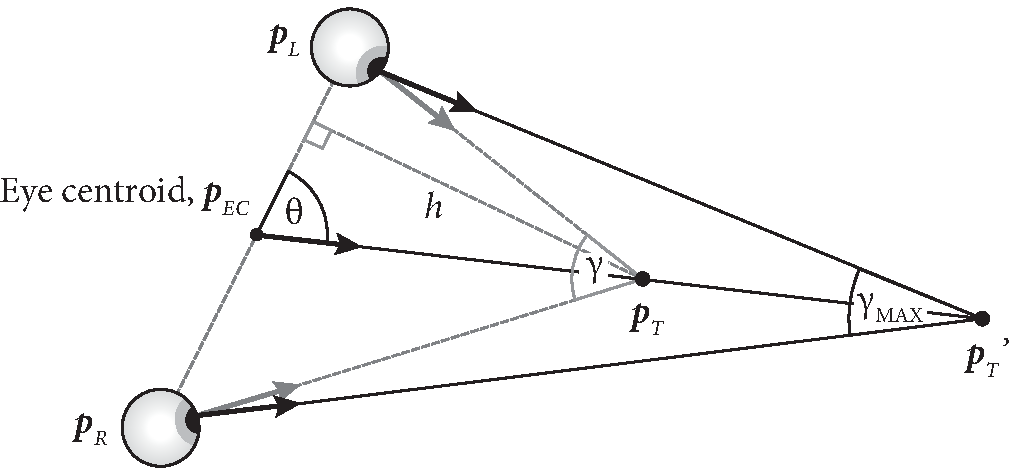
\includegraphics[width=0.85\textwidth]{stylizedgaze/Figures/CrosseyednessRemoval.pdf}
\caption{Our approach for reducing cross-eyedness in the target gaze pose.}
\label{fig:CrosseyednessRemoval}
\end{figure}

Our approach to remove cross-eyedness is illustrated in Figure~\ref{fig:CrosseyednessRemoval}. We measure cross-eyedness as the angle between the gaze directions of the two eyes, $\gamma$. Allowable cross-eyedness is defined by a threshold $\gamma_{MAX}$, which we leave at a default value of 0.002$^{\circ}$ for the examples in this paper.
We define the \textit{effective target position}, $\mathbf{p}_T'$, as the position behind the physical gaze target that the eyes can converge on without violating the cross-eyedness threshold. It is calculated by moving the target position away from the character to reduce $\gamma$ below the threshold value $\gamma_{MAX}$:
%
\begin{align}
\mathbf{p}_T' = \mathbf{p}_{EC} + \frac{\mathbf{p}_T - \mathbf{p}_{EC}}{||\mathbf{p}_T - \mathbf{p}_{EC}||} \frac{\sin(\theta + \gamma_{MAX}/2)}{sin(\gamma_{MAX}/2)}||\mathbf{p}_L - \mathbf{p}_{EC}||.
\end{align}
%
The above technique is effective at reducing cross-eyedness as shown in Figure~\ref{fig:CrosseyednessFixExample}.

The cross-eyedness removal technique is applied in a view-dependent manner; we may only apply it if the viewer cannot notice it from the current viewpoint.
If the viewer \emph{is} the gaze target, they may notice the character is looking a bit ``past'' them if cross-eyedness removal is applied.
Therefore, the cross-eyedness threshold $\gamma_{MAX}$ is adjusted based on the target viewing angle $\phi_T$, which we define as the angle between the viewer's gaze direction and the character's gaze direction at the target pose. We adjust $\gamma_{MAX}$ as follows:
%
\begin{align}
\label{eq:CrosseyednessFix}
\gamma\,'_{MAX} &= 2 OMR_{IN} + (\gamma_{MAX} - 2 OMR_{IN}) p_{\phi} \\
p_{\phi} &= \frac{\phi_T}{9.6W},~ 0 \le p_{\phi} \le 1 \nonumber
\end{align}
%
where $OMR_{IN}$ is inward OMR of the eye, and $W$ is the eye width parameter. The $9.6^{\circ}$ constant is derived from parameters of the viewing cone in which humans are able to detect subtle differences in gaze direction~\citep{argyle1976gaze}. We scale this value by $W$, as larger eyes may make such judgements easier. The viewing cone parameter, $p_{\phi}$, expresses the drop-off in judgement accuracy from the center of the cone toward the edge. We use $p_{\phi}$ to vary allowable cross-eyedness from the mechanical limit, $2 OMR_{IN}$, at the center of the cone, to $\gamma_{MAX}$ at the cone's edge and beyond.

\subsubsection{Eye Divergence}

\begin{figure}
\centering
\includegraphics[width=0.9\textwidth]{stylizedgaze/Figures/EyeDivergenceFixExample-small.pdf}
\caption{Example of eye divergence handling. Top: The VOR begins to move the left eye immediately on alignment. Bottom: Our model ensures that VOR begins eye movement only after the right eye has aligned.}
\label{fig:EyeDivergenceFixExample}
\end{figure}

A consequence of OMR asymmetry, eye divergence is handled by allowing the eyes to diverge during the gaze shift and imposing the principle that VOR for both eyes must trigger \emph{at the same time}. The leading eye will always overshoot the gaze target by a small amount and only begin moving in the opposite direction (due to VOR) when the trailing eye has reached the target. This behavior prevents the leading eye from aligning exactly with the target, as the accumulated overshoot rotation introduces an offset into the eye's target rotation. However, much like with cross-eyedness removal, this minor deviation from correct gaze convergence is difficult to detect. This technique is therefore an effective way of eliminating disconjugate eye movements as shown in Figure~\ref{fig:EyeDivergenceFixExample}.

As with cross-eyedness removal, eye divergence is applied in a view-dependent manner. The target overshoot introduced by the technique may be noticeable to the viewer at very low viewing angles, which we therefore adjust using the viewing cone parameter, $p_{\phi}$, that we defined in Equation~\ref{eq:CrosseyednessFix}. Specifically, we scale the outward OMR based on target viewing angle, $\phi_T$:
%
\begin{equation}
OMR_{OUT}' = OMR_{IN} + (OMR_{OUT} - OMR_{IN}) p_{\phi}
\end{equation}
%
This adjustment ensures that outward OMR will contract at low $\phi_T$, making the OMR symmetrical.

\subsection{Gaze Kinematics Adaptation}

\begin{figure*}
\centering
\includegraphics[width=1\textwidth]{stylizedgaze/Figures/GazeDynamicsExample1-small.pdf}
\caption{Gaze shifts with different gaze kinematics. Top: Original motion. The gaze shift contains the artifacts stuck eye, OMR-block, and eye retraction. Bottom: Our method. The artifacts of the original motion are reduced.}
\label{fig:GazeDynamicsExample}
\end{figure*}

Because most stylized characters do not have the same proportions and OMR as humans, we introduce a method for adapting the gaze shift kinematics based on these differences. The adaptation takes the form of scaling the gaze shift velocity. For our gaze shift model (Chapter~\ref{cha:GazeShiftModel}), that means changing the manner in which the peak eye velocity, $v_{\mathrm{max},E}$, is computed. However, the same adaptation can be applied to any gaze shift synthesis model that allows control over timing.

Our gaze kinematics adaptation is based on two key ideas. First, since stylized eyes can be asymmetric, each eye may need to cover a different angular distance as it rotates toward its OMR. We want to ensure that both eyes reach the OMR at the same time, thereby preventing artifacts such as \emph{stuck eye}. It follows that the eyes need to move at different velocities to reach the OMR at the same time. We define separate peak velocities, $v_{MAX,j}$, for each eye $j$. The second key idea is that stylized eyes are larger and therefore more massive than real human eyes, so they should move more slowly.

We use the anatomic parameters eye width, $W$, and muscle strength, $F$, to compute the peak eye velocities. As volume---and therefore mass---increases with $W^3$, both peak velocities are scaled down by the same factor. $F$ is used to compute an intermediate parameter $F'$, which varies depending on how much the head contributes to the gaze shift. We compute $F'$ as follows:
%
\begin{equation}
F' = ( 1 - \alpha_H ) W^3 + \alpha_H F.
\end{equation}
%
The parameter $\alpha_H$ specifies how much the head contributes to the gaze shift. When the head carries the eyes through most of the gaze shift (high $\alpha_H$), eye velocity should be lower in order to prevent the eyes from appearing improbably fast. When the head moves only a small distance, the eyes should move more quickly to prevent the gaze shift from appearing slow and sluggish.

To account for OMR asymmetry and prevent artifacts such as \textit{stuck eye}, we also need to apply a separate scaling factor to each velocity. Let $A_{OMR,j}$ be the distance that the eye $j$ can rotate before reaching its OMR, while $A_{MAX}$ is the highest rotational distance to the OMR for \emph{both} eyes. The peak velocity is scaled by $A_{OMR,j}/A_{MAX}$. This has the effect of slowing down the eye that has less to rotate, thus ensuring that both eyes reach the OMR at the same time.

Finally, we also introduce a velocity multiplier parameter, $\chi$, and apply it uniformly to eye and head velocities. This parameter can be used to make the character's gaze appear livelier or more languid, depending on their size, personality, and mood. By default, $\chi$ is set to $1$, although we use values between $1.2$ and $1.7$ for our stylized characters.
% NOTE: Clarified how the parameter might be used by explaining how we use it. -- Tomislav

We introduce these modifications to Equation~\ref{eq:AndristVmaxE} to create the following updated equation for calculating peak eye velocities:
%
\begin{equation}
v_{MAX,j} = \frac{F}{W^3}( \frac{2}{75} A_{MAX} + \frac{1}{6} ) \frac{A_{OMR}}{A_{MAX}} \chi v_0%+ 3 \delta V_{MAX,H}
\end{equation}
%
The first, third, and fourth terms implement our modifications to gaze kinematics. The second term speeds up or slows down the eyes depending on eye movement amplitude and is similar to the term used by the original model to calculate the peak velocity, except that $A_{MIN}$ is replaced by $A_{MAX}$.
%The rightmost term $3 \delta v_{MAX,H}$ addresses an issue with the original gaze model. For certain rare gaze shifts, the angle $\delta$ between eye and head rotation directions may become much greater than 0; eyes could even end up moving in the opposite direction of the head. In these cases, the head is slowing down the eyes rather than helping them reach the target, so the above term speeds up the eyes to compensate for the opposing head rotation.
% Since this is a bugfix of the original model, maybe it doesn't need to be here? It muddles the story somewhat, and takes up space...

Using the above method for calculating peak eye velocities reduces the artifacts related to gaze kinematics, producing gaze shifts that appear smoother and more lifelike. The stuck eye artifact is largely eliminated; the amount of time spent in the state of OMR-block is greatly reduced; and the VOR causes less eye retraction (Figure~\ref{fig:GazeDynamicsExample}). The eye retraction cannot be completely eliminated, as some VOR must occur to achieve the specified head alignment and thus produce desired communicative effects.

\subsection{Gaze-evoked Eye Blinks}

\begin{figure}
\centering
\includegraphics[width=0.85\textwidth]{stylizedgaze/Figures/GazeEvokedBlinkVOR-small.pdf}
\caption{A gaze-evoked eye blink during the VOR phase. The blink conceals the retraction in the left eye.}
\label{fig:GazeEvokedBlinkVOR}
\end{figure}

As described in Section~\ref{sec:GazeShiftSecondary}, our gaze shift model also incorporates gaze-evoked eye blinks. At the beginning of the gaze shift, it is probabilistically determined whether or not a gaze-evoked eye blink will occur.
The timing of the blink is deterministic---if generated, the blink occurs immediately at the start of the gaze shift.
As part of our efforts to reduce gaze animation artifacts, we propose introducing more variability into the timing of gaze-evoked blinks. Specifically, we schedule the blinks to co-occur with potential eye retraction artifacts in order to conceal them by the character's eyelids (Figure~\ref{fig:GazeEvokedBlinkVOR}).

Our implementation generates a gaze-evoked eye blink at the start of the gaze shift, using the same probabilistic method as in the baseline model. However, when determining the timing of the blink, we estimate the duration of the VOR phase of the gaze shift, $T_{VOR}$, and the time when the VOR phase will begin, $t_{VOR}$. If $T_{VOR}$ is greater than a threshold value, then the gaze-evoked blink is scheduled to begin at $t_{VOR} - 0.35T_{B}$, where $T_B$ is the duration of the eye blink (generated probabilistically), and $0.35T_B$ is the time when the eyes are fully closed.
